\documentclass[12pt]{article}
\usepackage[english]{babel}
\usepackage[T1]{fontenc}
\usepackage[nopatch=eqnum]{microtype}
\usepackage{setspace}
\usepackage{parskip}
\usepackage{titling}
\usepackage{titlesec}
\usepackage{fourier-otf}
\usepackage{tgschola}
\usepackage[hidelinks]{hyperref}
\usepackage{fontspec}
\usepackage{fancyhdr}
\usepackage{etoolbox}
\usepackage{lastpage}
\usepackage{sectsty}
\usepackage{adforn}
\usepackage{amsmath}
\usepackage{graphicx}
\usepackage{svg}
\usepackage{geometry}
\usepackage{booktabs}
\usepackage{siunitx}
\usepackage{longtable}
\usepackage{sepfootnotes}
\usepackage[hang,flushmargin]{footmisc}
\geometry{
    a4paper,
    left=30mm,
    right=30mm,
    top=25mm,
    bottom=20mm
}
\usepackage{hyperref}

\setlength{\headheight}{15pt}

% enable for word export
% \tolerance=1
% \emergencystretch=\maxdimen
% \hyphenpenalty=10000
% \hbadness=10000

% Custom font import
\setmainfont{Calluna}[
    Path=./Calluna/,
    Extension = .otf,
    UprightFont=*-Regular,
    BoldFont=*-Bold,
    ItalicFont=*-It,
    BoldItalicFont=*-BoldIt
]

\settowidth{\thanksmarkwidth}{*}
\setlength{\thanksmargin}{1.3em}
\makeatletter
  \long\def\@makefntext#1{\leavevmode%
    \@thefnmark)\hspace{1em}\nobreak
    \relax#1%
  }
\makeatother

% Header and footer.
\fancyhead[L]{\nouppercase\leftmark}
\fancyhead[R]{\thepage}
\fancyfoot[R]{\hfill}
\fancyfoot[C]{}

% Custom header-less plain first page.
\fancypagestyle{plain}{ 
    \fancyhf{}
    \renewcommand{\headrulewidth}{0pt}
    \fancyfoot[R]{\hfill}
}

% Body styling.
%\renewcommand{\thepart}{\Roman{part}}
\sectionfont{\centering\textsc}
\subsectionfont{\centering}
\subsubsectionfont{\textit}
\renewcommand{\thesection}{\Roman{section}}
\renewcommand\thesubsection{\normalfont\textbf\Alph{subsection}}
\renewcommand\thesubsubsection{\normalfont\textbf{\textit{\arabic{subsubsection}}}}
\onehalfspacing

\newcommand{\Star}[1]{#1\ensuremath{^*}\kern-\scriptspace}
\newcommand{\PStar}[1]{\ensuremath{^*}\kern-\scriptspace #1}
\let\xn\xnote
\newfootnotes{x}
\let\fn\xnotecontent

\newcommand{\id}{Ibid.}
\newcommand{\sr}[1]{(`\textit{#1}')}

% Change footnote size to match body.
%\renewcommand{\footnotesize}{\fontsize{}{14.4pt}\selectfont}

% Prevent footnote spillage.
\interfootnotelinepenalty=10000

% Change footnote top margin.
\addtolength{\skip\footins}{2pc plus 5pt}

% Footnote text formatting.
\makeatletter
\renewcommand{\@makefntext}[1]{%
  \setlength{\parindent}{0pt}%
  \begin{list}{}{%
    \setlength{\labelwidth}{1.5em}%
    \setlength{\leftmargin}{\labelwidth}%
    \setlength{\labelsep}{3pt}%
    \setlength{\itemsep}{0pt}%
    \setlength{\parsep}{0pt}%
    \setlength{\topsep}{0pt}%
    \footnotesize}%
  \item[\@makefnmark\hfil]#1%
  \end{list}%
}
\makeatother

% Prevent footnote spillage.
\interfootnotelinepenalty=10000

% Change space between footnotes.
\setlength{\footnotesep}{0.75\baselineskip}

% ----------------------------------------------------------

\begin{document}
%TC:ignore
%TC:ignore
% Don't include footnotes in word count.

% Footnotes.
% \fn{}{\iit{}.}

% INTRODUCTION
\fn{1-1}{Chief Justice Susan Kiefel, `The academy and the courts: What do they mean to each other today?' (2020) 44(1) \textit{Melbourne University Law Review} 447, 451. See also Neil Duxbury, `Better read when dead?' (2000) 32 \textit{Amicus Curiae} 25.}

\fn{1-2}{Richard A Posner, `The Judiciary and the Academy: A Fraught Relationship' (2010) 29(1) \textit{University of Queensland Law Journal} 13, 15-6.}

\fn{1-3}{`A Conversation with Chief Justice Roberts', \textit{Fourth Circuit Court of Appeals: 77th Annual Conference} (C-Span, 2011) 0:30:50-0:31:10 <\url{https://www.c-span.org/video/?300203-1/conversation-chief-justice-roberts}>.}

\fn{1-4}{See, eg, Kiefel (n 1) 455; Justice Michael Kirby, `Welcome to Law Reviews' (2002) 26(1) \textit{Melbourne University Law Review} 1, 6-11; Chief Justice Robert French, `Judges and Academics - Dialogue of the Hard of Hearing' (Speech, Australian Academy of Law, 30 October 2012) 14-5. But some academics find this direction concerning. See, eg, John Gava, `Law Reviews: Good for Judges, Bad for Law Schools?' (2002) 26(3) \textit{Melbourne University Law Review} 560, 575-6.}

\fn{1-5}{Sir Anthony Mason, `Future Directions in Australian Law' (1987) 13(3) \textit{Monash University Law Review} 149, 154; Justice Stephen Gageler, `The Coming of Age of Australian Law' in Barbara McDonald, Ben Chen and Jeffrey Gordon (eds), \textit{Dynamic and Principled} 8, 23-7}

\fn{1-6}{\textit{Visy Paper Pty Ltd v Australian Competition and Consumer Commission} (2003) 216 CLR 1, 25 [75] \sr{Visy}.}

\fn{1-7}{\textit{Australian Crime Commission v Stoddart} (2011) 244 CLR 554, 605-7 [132]-[135] \sr{Stoddart}.}

\fn{1-8}{Ibid 607 [135].}

\fn{1-9}{French (n 4) 9, 17-8.}

\fn{1-10}{Ibid.}

% SECTION 2
\fn{2-1}{See, eg, Brian T Detweiler, `May It Please the Court: A Longitudinal Study of Judicial Citation to Academic Legal Periodicals' (2020) 39(2) \textit{Legal Reference Services Quarterly} 87, 114-8. Detweiler uses a variety of wildcard searches in Lexis as a basic method for extracting journal articles from judgments. Joshua D Baker, `Relics or Relevant: The Value of the Modern Law Review' (2009) 111(3) \textit{West Virginia Law Review} 919, 928. Finding a noticeable decrease in the number of citations between 1971 to 1998. Baker also finds prestigious law journals to be cited more frequently. David L Schwartz and Lee Petherbridge, `The Use of Legal Scholarship by the Federal Courts of Appeals: An Empirical Study' (2011) 96(6) \textit{Cornell Law Review} 1345, 1361. Contrary to Baker, Schwartz and Lee found an increase in the number of citations to law journals between 1950 and 2008. This divergence in outcome might cause legal commentators who see these scientometric studies as unfit for purpose. Richard G Kopf, `Do Judges Read the Review - A Citation-Counting Study of the Nebraska Law Review and the Nebraska Supreme Court, 1972-1996' (1997) 76 \textit{Nebraska Law Review} 708, 717, 719-20. Former District Court Judge Kopf formulates a test for determining the qualitative impact of a citation by evaluating whether the relying paragraph directly mentions or follows the citation. On this method, see also Xiaodan Zhu et al, `Measuring academic influence: Not all citations are equal' (2014) 66(2) \textit{Journal of the Association for Information Science and Technology} 408, 413.}

\fn{2-2}{Kopf (n 11) 710. But see Lee Petherbridge and David L. Schwartz, `An Empirical Assessment of the Supreme Court's use of Legal Scholarship' (2012) 106(3) \textit{Northwestern University Law Review} 995, 1000-4. ``Content analysis'' refers to the practice of precisely determining the exact treatment of a journal citation through a process of manual review.}

\fn{2-3}{See generally Andrew Lynch, `Judicialization of Politics: The Interplay Of Institutional Structure, Legal Doctrine And Politics on the High Court of Australia', (2013) 34(2) \textit{Adelaide Law Review} 465, 466-7.}

\fn{2-3a}{See, eg, Brian Opeskin and Gabrielle Appleby, `Responsible Jurimetrics:
A Reply to Silbert’s Critique of the Victorian Court of Appeal' (2020) 94(12) \textit{Australian Law Journal} 923. Alan L. Tyree, `Fact Content Analysis of Case Law: Methods and Limitations' (1981) 22(1) \textit{Jurimetrics} 1, 2.}

\fn{2-3b}{See \textit{LOI n° 2019-222 du 23 mars 2019 de programmation 2018-2022 et de réforme pour la justice} (France) JO, 24 March 2019, art 33.}

\fn{2-3ba}{Russell Smyth, `Empirical studies of judicial behaviour and decision-making in Australian and New Zealand courts' in Nuno Garoupa, Lydia Tiede, and Rebecca D. Gill (eds), \textit{The Comparative Empirical Conundrum: Understanding High Court Behavior} (University of Virginia Press, 2020) 1, 13-4.}

\fn{2-3bb}{Federal Circuit and Family Court of Australia (Division 2), `Statement to Damien Carrick, ABC Law Report' (Media Release, 1 August 2022).}

\fn{2-3bc}{See, eg, Tonja Jacobi, Zoë Robinson and Patrick Leslie, `Querying the Gender Dynamics of Interruptions at Australian Oral Argument' (2020) 4 \textit{University of New South Wales Law Journal Forum} 1, 18-9. In response to an article by Amelia Loughland examining the influence gender carries on whether a High Court justice is likely to be interrupted during oral arguments, the authors carried out a regression analysis of the provided data and concluded that the results were of no statistical significance (ie, a \textit{p}-value $>$ 0.05).}

\fn{2-3c}{Australian Law Reform Commission, \textit{Judicial Impartiality} (Report No 138, December 2021) 495-6.}

\fn{2-4}{See, eg, Russell Smyth and Ingrid Nielsen, `The Citation Practices of the High Court of Australia, 1905-2015' (2019) 47(4) \textit{Federal Law Review} 655; Russell Smyth, `Other than ``Accepted Sources of Law''?: A Quantitative Study of Secondary Source Citations in the High Court' (1999) 22(1) \textit{University of New South Wales Law Journal} 19 \sr{Other than ``Accepted Sources of Law''?}; Russell Smyth, `What Do Trial Judges Cite? Evidence From the New South Wales District Court' (2018) 41(1) \textit{University of New South Wales Law Journal} 211 \sr{What Do Trial Judges Cite?}.}

\fn{2-5}{Smyth and Nielsen (n 20) 662-3.}

\fn{2-5a}{Ibid. See also Ingrid Nielsen and Russell Smyth, `One Hundred Years of Citation of Authority on the Supreme Court on New South Wales' (2008) 31(1) \textit{University of New South Wales Law Journal} 189, 195. The authors review trends over 100 years with data sampled from only 10 cumulative years.}

\fn{2-6}{G. S. Maddala, `Selectivity Problems in Longitudinal Data' (1978) 30/31 \textit{Annales de l'inséé} 423, 429. See especially from ``sample selectivity'' and truncation bias onwards.}

\fn{2-7}{See, eg, Smyth, \textit{What Do Trial Judges Cite?} (n 20) 229.}

\fn{2-8}{See especially Russell Smyth, ‘Who Publishes in Australia’s Top Law Journals’ (2012) 18(1) \textit{University of New South Wales Law Journal} 201, 219. The author concludes with: “[s]tudies of this sort could fruitfully be the subject of future research, where the focus of the research is on the influence ... on legal scholarship and reasoning in courts’ decisions in an Australian context”.}

\fn{2-9}{Lynch (n 13).}

\fn{2-10}{Lyria Bennett Moses, Nicola Gollan and Kieran Tranter, ‘The Productivity Commission:
a different engine for law reform?’ (2015) 24(4) \textit{Griffith Law Review} 657, 667-8.}

\fn{2-11}{For criticism on the use of empirical methods to determine academic impact, see Kathy Bowrey, ‘A Report into Methodologies Underpinning Australian Law Journal Rankings’ (Research Paper No 2016-30, University of New South Wales Faculty of Law, Prepared for the Council of Law Deans, 18 February 2016) 37-8.}

\fn{2-12}{Martin Szomszor, David A Pendlebury and Jonathan Adams, `How much is too much? The difference between research
influence and self-citation excess' (2020) 123(2) \textit{Scientometrics} 1119, 1120-1.}

\fn{2-12a}{Bowrey (n 28) 38.}

\fn{2-12b}{Ibid.}

\fn{2-13}{Jacobi, Robinson and Leslie (n 18) 13-5.}

\fn{2-14}{Carl T Bergstrom, Jevin D West and Marc A Wiseman, `The Eigenfactor™ Metrics' (2008) 28(45) \textit{Journal of Neuroscience} 11433.}

\fn{2-15}{See Lutz Bornmann and Hans-Dieter Daniel, `What Do We Know About the \textit{h} Index?' (2007) 58(9) \textit{Journal of the American Society for Information Science and Technology} 1, 1.}

% SECTION 3.1

\fn{3-1}{Robin Creyke, et al, \textit{Laying Down the Law} (LexisNexis Butterworths, 11\textsuperscript{th} ed, 2020) 228-30.}

\fn{3-2}{KR Chowdhary, \textit{Fundamentals of Artificial Intelligence} (Springer Nature, 2020) 604.}

\fn{3-3}{But see LT Olsson, \textit{Guide to Uniform Production of Judgments} (Australian Institute of Judicial Administration, 2\textsuperscript{nd} ed, 1999). Attention should be drawn to the divergence of citation formats from those outlined in uniform guides.}

\fn{3-4}{Melbourne University Law Review Association, \textit{Australian Guide to Legal Citation} (2020).}

\fn{3-5}{Ibid.}

\fn{3-6}{For an overview of regular expressions and the application of regular expressions to legal text more generally, see `Lexical Analysis Using Regular Expressions for Information Retrieval from a Legal Corpus' in Patricia Pesado and Gustavo Gil (eds), \textit{Computer Science – CACIC 2021} (Springer Nature, 2022) 312.}

\fn{3-7}{\textit{BarNet Jade} (Web Page, 16 October 2022) <\url{https://jade.io/}> \sr{Jade}.}

\fn{3-8}{\textit{BarNet Jade}, `Jade Browser' (Web Page, 16 October 2022) <\url{https://jade.io/search/collection=HCA:effective.since=883573200000:effective.until=1664114400000:order1.effectivedateasc=desc}>.}

\fn{3-9}{See, eg, Horacio Paggi et al, `Towards the definition of an information quality metric for information fusion models' (2021) 89 \textit{Computers and Electrical Engineering} 1.}

\fn{3-10}{Google, `General recommended practices for AI', \textit{Responsible AI practices} (Web Page, 16 October 2022) archived at <\url{https://archive.ph/czKPH}>.}

\fn{3-11}{Ibid.}

\fn{3-12}{Alireza Mansouri et al, `Named Entity Recognition Approaches' (2008) 8(2) \textit{International Journal of Computer Science and Network Security} 339.}

\fn{3-13}{See, eg, Gabriel Zingle et al, ‘Detecting Suggestions in Peer Assessments’ (Conference Paper, Proceedings of the International Conference on Educational Data Mining, 2 July 2019) 475.}
\fn{3-14}{See, eg, \textit{The Queen v Abdirahman-Khalif} (2020) 271 CLR 265, 295 [50]. In footnote 29, the Court references Lynch, McGarrity and Williams by surname.}

\fn{3-15}{For an example of data enrichment in practice, see Stainslaw AB Stane and Mariusz Zytniewsk, `Normative Multi-Agent Enriched Data Mining to Support E-Citizens' in Longbing Cao (ed), \textit{Data Mining and Multi-agent Integration} (Springer, 1\textsuperscript{st} ed, 2009) 321.}

\fn{3-16}{\textit{Australasian Legal Information Institute}, `LawCite Overview', \textit{What is LawCite?} (Web Page, 26 June 2014) archived at <\url{https://archive.ph/FFfop}>.}

\fn{3-17}{See, eg, \textit{Australasian Legal Information Institute}, `Formularism and Tort Law', \textit{Cases and Articles Cited} (Web Page, 20 October 2022) archived at <\url{https://archive.ph/tAv74}>.}

\fn{3-18}{Suzanne Scotchmer, `Standing on the Shoulders of Giants: Cumulative Research and the Patent Law' (1991) 5(1) \textit{Journal of Economic Perspectives} 29.}

\fn{3-19}{John PA Ioannidis, `Why Most Published Research Findings Are False' (2005) 2(8) \textit{PLoS Medicine} 696, 696, 699-700. See also Mark A Hall and Ronald F Wright, `Systematic Content Analysis of Judicial Opinions' (2008) 96(1) \textit{California Law Review} 63, 105-6.}

\fn{3-20}{Jason M Chin et al, `Improving the Credibility of Empirical Legal Research: Practical Suggestions for Researchers, Journals and Law Schools' (2021) 3(2) \textit{Law, Technology and Humans} 107, 108.}

\fn{3-21}{See, eg, \textit{Jade} (n 41). See also \textit{Australasian Legal Information Institute} (Web Page, 20 October 2022) <\url{https://www.austlii.edu.au/}>.}

\fn{3-22}{Chin et al (n 54) 119-20.}

\fn{3-23}{The dataset used in this study is publicly accessible, see \textbf{TODO: get link}.}

% SECTION 3.1

\fn{3b-0}{See Felicity Bell, `Empirical research in law' (2016) 25(2) \textit{Griffith Law Review} 262, 267.}

\fn{3b-4}{Norman Blaikie, \textit{Analysing Quantitative Data} (SAGE Publications, 2003) 39-40.}

\fn{3b-5}{Blaikie (n 59) 80.}

\fn{3b-5aa}{See \textit{Farah Constructions Pty Ltd v Say-Dee Pty Ltd} (2007) 230 CLR 89, 150 [134], affd \textit{Hill v Zuda Pty Ltd} (2022) 96 ALJR 540, 545 [25].}

\fn{3b-5a}{Bornmann and Daniel (n 34) 1.}

\fn{3b-5b}{John Clauser was awarded the 2022 Nobel Prize in Physics with a respectable but unextraordinary \textit{h}-index of 29. See, eg, Lutz Bornmann and Werner Marx, `The h index as a research performance indicator' (2011) 37(3) \textit{European Science Editing} 77, 77-8. But see JE Hirsch, `Does the h index have predictive power?' (2007) 104(49) \textit{Proceedings of the National Academy of Sciences of the United States of America} 19193, 19197.}

\fn{3b-5bb}{See Jingda Ding, Chao Liu and Goodluck Asobenie Kandonga, `Exploring the limitations of the h-index and h-type indexes in measuring the research performance of authors' (2020) 122(3) \textit{Scientometrics} 1303, 1305.}

\fn{3b-6}{P McCullagh and JA Nelder, \textit{Generalized Linear Models} (Chapman and Hall, 2\textsuperscript{nd} ed, 1989) 3-4.}

\fn{3b-7}{Ibid.}

\fn{3b-7a}{Judea Pearl, \textit{Causality} (Cambridge University Press, 2\textsuperscript{nd} ed, 2009) 134.}

\fn{3b-8}{Simon Rogers and Mark Girolami, \textit{A First Course in Machine Learning} (CRC Press, 2\textsuperscript{nd} ed, 2017) 41-3.}

\fn{3b-8a}{For an overview of data fitting practices including regularised least squares optimisation and maximum likelihood estimation, see Rogers and Girolami (n 68) 34, 70. See also Jared Wilber, `A Visual Introduction To (Almost) Everything You Should Know', \textit{Linear Regression} (Web Page, September 2022) archived at <\url{https://archive.ph/Oh5p2}>.}

\fn{3b-9}{Rogers and Girolami (n 68) 43.}

\fn{3b-10}{Ibid.}

\fn{3b-11}{See Sheldon M Ross, \textit{Introduction to Probability Models} (Academic Press, 12\textsuperscript{th} ed, 2019) 27.}

\fn{3b-12}{AJ Dobson and AG Barnett, \textit{An introduction to generalized linear models} (CRC Press, 3\textsuperscript{rd} edition, 2018) 197.}

\fn{3b-13}{Ibid. See also Joop J Hox, Mirjam Moerbeek and Rens van de Schoot, \textit{Multilevel Analysis: Techniques and Applications} (Taylor \& Francis Group, 2\textsuperscript{nd} ed, 2010) 151.}

\fn{3b-14}{Dobson and Barnett (n 73) 199.}

\fn{3b-15}{Mirko Bagaric and James McConvill, `The High Court and the Utility of Multiple
Judgments' (2005) 1(1) \textit{High Court Quarterly Review} 13, 21.}

\fn{3b-16}{The coefficients for the GLMM are estimated with random intercepts grouping data points for each justice (n=21) and year (n=24). For similar identification of non-independent variables, see Jacobi, Robinson and Leslie (n 18) 14. At footnote 51.}

\fn{3b-17}{Hox, Moerbeek and Schoot (n 78) 3-5. See also UCLA: Statistical Consulting Group, `Introduction to Generalized Linear Mixed Models', \textit{Statistical Methods and Data Analytics} (Web Page, April 2022) archived at <\url{https://archive.ph/a9T2s}>.}

\fn{3b-18}{Hox, Moerbeek and Schoot (n 78) 12.}

\fn{3b-19}{Hox, Moerbeek and Schoot (n 78) 13.}

\fn{3b-20}{Hox, Moerbeek and Schoot (n 78) 152. See also UCLA (n 78).}

\fn{3b-21}{Ronald L Wasserstein and Nicole A Lazar, `The ASA Statement on p-Values: Context, Process, and Purpose' (2016) 70(2) \textit{The American Statistician} 129, 131.}

\fn{3b-22}{Herman Aguinis, Matt Vassar and Cole Wayant, `On reporting and interpreting statistical significance and p values in medical research' (2019) 26(2) \textit{BMJ Evidence-Based Medicine} 39.}

\fn{3b-23}{See John PA Ioannidis et al, `A standardized citation metrics author database annotated for scientific field' (2019) 17(8) \textit{PLoS Biology} e3000384:1-6.}

\fn{3b-24}{See generally Avrim Blum, John Hopcroft and Ravindran Kannan, \textit{Foundations of Data Science} (Cambridge University Press, 2020) 97.}

\fn{3b-25}{Previous studies have found that judges on the High Court and Federal Court publish most actively in the \textit{Australian Law Journal}, see Russell Smyth, `Judges and Academic Scholarship: An Empirical Study of the Academic Publication Patterns Of Federal Court and High Court Judges' (2002) 2(2) \textit{Queensland University of Technology Law and Justice Journal} 198, 209.}

\fn{3b-26}{\textit{Forge v Australian Securities and Investments Commission} (2006) 228 CLR 45, 130 [216]. At footnote 271.}

\fn{3b-27}{Ernst Willheim, `Review of Australian Public Law Developments' (2006) 30(1) \textit{Melbourne University Law Review} 269.}

\fn{3b-28}{Ibid 278; Adrienne Stone, `The Limits of Constitutional Text and Structure: Standards of Review and the Freedom of Political Communication' (1999) 23(3) \textit{Melbourne University Law Review} 668.}

\fn{3b-28a}{\textit{Clubb v Edwards} (2019) 267 CLR 171, 332 [467]. At footnote 599.}

\fn{3b-29}{\textit{Brown v Tasmania} (2017) 261 CLR 328, 465 [430]. At footnote 454.}

\fn{3b-30}{Kurt Bryan and Tanya Leise, `The \$25,000,000,000 Eigenvector: The Linear Algebra behind Google' (2006) 48(3) \textit{SIAM Review} 569, 571.}

\fn{3b-31}{Blum, Hopcroft and Kannan (n 85) 97.}

\fn{3b-32}{Bryan and Leise (n 92) 571.}

\fn{3b-33}{Sergey Brin and Lawrence Page, `The anatomy of a large-scale hypertextual Web search engine' (1998) 30(1-7) \textit{Computer Networks and ISDN Systems} 109-10.}

\fn{3b-34}{Bryan and Leise (n 92) 580. By convention, $\upalpha$ is set to a value of $0.85$, see Brin and Page (n 95) 109.}

\fn{3b-35}{The mathematical basis for this algorithm lies in the formulation of a stochastic matrix that calculates the stationary probabilities for a random walker, see generally Gilbert Strang, \textit{Linear Algebra and Learning from Data} (Cambridge University Press, 2019) 312-18.}

\fn{3b-36}{The founders of Google describe the ability to teleport as a `damping factor', see Brin and Page (n 95) 109-10.}

\fn{3b-37}{Massimo Franceschet, `PageRank: Standing on the shoulders of giants' (2011) 54(6) \textit{Communications of the ACM} 92, 94.}

\fn{3b-38}{Ibid 95.}

\fn{3b-39}{Ibid.}

\fn{3b-40}{Bryan and Leise (n 92) 580.}

\fn{3b-41}{Ibid.}

\fn{3b-42}{Brin and Page (n 95) 109-10.}

\fn{3b-43}{Ibid. For a brief overview of the power method to compute the left eigenvector of large sparse matrices, see Mung Chiang, \textit{Networked Life: 20 Questions and Answers} (Cambridge University Press, 2012) 49-52.}


% SECTION 4

\fn{4-1}{Andrew Lynch, `The Gleeson Court on Constitutional Law: An
Empirical Analysis of Its First Five Years' (2003) 26(1) \textit{University of New South Wales Law Journal} 32, 35-6.}

\fn{4-2}{Joanne Sherman, `Council of Chief Justices Electronic Appeals Project —The Consultant’s Overview' (1998) 36 \textit{Computers \& Law} 29, 29-30.}

\fn{4-3}{Joel B Grossman, `Social Backgrounds and Judicial Decision-Making' (1966) 79(8) \textit{Harvard Law Review} 1551, 1563.}

\fn{4-4}{Ibid. See also Tonja Jacobi, Zoë Robinson and Patrick Leslie, `Comparative Exceptionalism? Strategy and Ideology in the High Court of Australia' \textit{American Journal of Comparative Law} (forthcoming), 27; Russell Smyth, `Explaining Voting Patterns on the Latham High Court 1935-50' (2002) 26(1) \textit{Melbourne University Law Review} 88, 103.}

\fn{4-5}{See generally Salvador García, Julián Luengo and Francisco Herrera, \textit{Data Preprocessing in Data Mining} (Springer, 2014) 46.}

\fn{4-6}{Fred R Shapiro, `The Most-Cited Law Review Articles' (1985) 73(5) \textit{California Law Review} 1540, 1543.}

\fn{4-7}{Ronen Perry, `The Relative Value of American Law Reviews: A Critical Appraisal of Ranking Methods' (2006) 11(1) \textit{Virginia Journal of Law and Technology} 1, 24.}

\fn{4-8}{Ibid; see also James Leonard, `Seein' the Cites: A Guided Tour of Citation Patterns in Recent American Law Review Articles' (1990) 34(2) \textit{Saint Louis University Law Journal} 181, 191.}

\fn{4-9}{Neil R Smalheiser and Vetle I Torvik, `Author Name Disambiguation' (2009) 43(1) \textit{Annual Review of Information Science and Technology} 6-1.}

\fn{4-10}{Ibid.}

\fn{4-11}{In 2016, Associate Professor Yvonne Corcoran-Nantes found more than 80\% of women take their husband's name after marriage. It is well-within contemplation that such practices disproportionately skew these types of longitudinal studies. See Sara Garcia, `Most Australian women still take husband's name after marriage, professor says', \textit{ABC News} (Web Page, 26 Apr 2016) archived at <\url{https://archive.ph/PxuKQ}>. See generally Anne F Young, Jennifer R Powers and Sandra L Bell, `Attrition in longitudinal studies: who do you lose?' (2006) 30(4) \textit{Australian and New Zealand Journal of Public Health} 353, 360.}

\fn{4-12}{ORCID, `About ORCID' (Web Page, 12 November 2022) archived at <\url{https://archive.ph/WYBDk}>.}

\fn{4-13}{Google, `About' \textit{Google Scholar} (Web Page, 12 November 2022) archived at <\url{https://archive.ph/rwv1N}>.}

% SECTION 5
\fn{5-1}{Including Toohey (1987), Gaudron (1987), McHugh (1989), Gummow (1995), and Kirby (1996) JJ.}

\fn{5-2}{See, eg, Benedict Sheehy and John Dumay, `Examining Legal Scholarship in Australia: A Case Study' (2021) 49(1) \textit{International Journal of Legal Information} 32, 34. see also Justice PW Young, ``Current issues'' (1998) 72(4) \textit{Australian Law Journal} 249, 254.}

\fn{5-3}{Ranked A* according to the Excellence in Research for Australia rankings (discontinued), see Australian Research Council, `2010 Final Journal List 100310 FOR WEBSITE', (Web Page, 19 November 2022) archived at <\url{https://archive.ph/WW12R}> (`ARC'). Ranked 44 in the United Kingdom with a combined score of (0.92) by the Washington and Lee University, see Washington and Lee University School of Law, `W\&L Law Journal Rankings', (Web Page, 19 November 2022) archived at <\url{https://archive.ph/D0SzE}>.}

\fn{5-4}{Ranked B according to the Excellence in Research for Australia rankings (discontinued), see ARC (n 119).}

\fn{5-5}{Ranked A according to the Excellence in Research for Australia rankings (discontinued), see ARC (n 119).}

\fn{5-6}{Smyth and Nielsen (n 20) 677-8.}

\fn{5-7}{Kevin Gray, `Property in Thin Air' (1991) 50(2) \textit{Cambridge Law Journal} 252; John W Salmond, `Citizenship and Allegiance' (1902) 18(1) \textit{Law Quarterly Review} 49.}

\fn{5-8}{See, eg, Smyth and Nielsen (n 20) 677.}

\fn{5-9}{JD Heydon, \textit{Cross on Evidence} (Lexis Nexis, 13\textsuperscript{th} ed, 2021).}

\fn{5-10}{FW Maitland, \textit{Equity} (Cambridge University Press, 1936).}

\fn{5-11}{OW Holmes Jr, \textit{The Common Law} (Little, Brown \& Company, 1881).}

\fn{5-12}{Smyth (n 25).}

\fn{5-13}{Ibid 241-2.}

% SECTION 6
\fn{6-1}{High Court of Australia, `Operation of the High Court', \textit{About} (Web Page, 13 November 2022) archived at <\url{https://archive.ph/LYu1x}>.}

\fn{6-2}{Graeme Orr, `Verbosity and richness: current trends in the craft of the High Court' (1998) 6(3)  \textit{Torts Law Journal} 291, 294.}

\fn{6-3}{(2020) 270 CLR 152, \sr{Love}.}

\fn{6-4}{Ibid 192 [81].}

\fn{6-5}{See Evan Young, ``A very bad thing': Peter Dutton slams High Court's Aboriginal `aliens' ruling' (Web Page, 13 February 2020) archived at <\url{https://archive.ph/9j87P}>. For an attempt by the government at overturning \textit{Love}, see Transcript of Proceedings, \textit{Montgomery v Minister for Immigration, Citizenship, Migrant Services and Multicultural Affairs} (High Court of Australia, Keane J, 29 November 2021).}

\fn{6-6}{(2019) 267 CLR 560 \sr{Mann}.}

\fn{6-7}{Ibid 618 [149].}

\fn{6-8}{\textit{Mann} (n 135) 645 [205].}

\fn{6-9}{Goh Yihan and Andrew Phang  `A Statistical Analysis of the Influence of the Journal of Contract Law in Commonwealth Court Decisions' 35(14) \textit{Journal of Contract Law} 14, 23.}

\fn{6-10}{For similar impact trends, see Smyth, \textit{Other than ``Accepted Sources of Law''?} (n 20) 36-7; Russell Smyth, `Academic Writing and the Courts: A Quantitative Study of the Influence of Legal and Non-Legal Periodicals in the High Court' (1998) 17(2) \textit{University of Tasmania Law Review} 164, 177.}

\fn{6-11}{Unlike the practice of assigning draft opinion writing to clerks in the United States Supreme Court, writing judgments tends not to be delegated to associates in the High Court, see Andrew Leigh, `Behind the Bench' (2000) 25(6) \textit{Alternative Law Journal} 295, 297. See also Andrew Lynch, `Individual Judicial Style and Institutional Norms' in Gabrielle Appleby and Andrew Lynch (eds) \textit{The Judge, the Judiciary and the Court} (Cambridge University Press, 2021) 214-5.}

\fn{6-12}{For example regression analyses of citations in New Zealand, see Russell Smyth, `Case complexity and citation to judicial authority: some empirical evidence from the New Zealand Court of Appeal' (2003) 10(1) \textit{Murdoch University Electronic Journal of Law}. But see Russell Smyth `Explaining historical dissent rates in the high court of Australia' (2003) 41(2) \textit{Commonwealth and Comparative Politics} 83.}

\fn{6-13}{Matthew Groves and Russell Smyth, `A Century of Judicial Style: Changing Patterns In Judgment Writing on the High Court 1903–2001' (2004) 32(2) \textit{Federal Law Review} 255, 262.}

\fn{6-14}{\textit{1903} (Cth) s 23(1) \sr{Judiciary Act}.}

\fn{6-15}{Benjamin Alarie, Andrew Green and Edward M Iacobucci, `Panel selection on high courts' (2015) 65(4) \textit{University of Toronto Law Journal} 335, 359.}

\fn{6-16}{Justice Susan Kiefel , `The individual judge' (2014) 88(8) \textit{Australian Law Journal} 554, 558.}

\fn{6-17}{Andrew Lynch and George Williams, `The High Court on Constitutional Law: The 2014 Statistics' (2015) 38(3) \textit{University of New South Wales Law Journal} 1078, 1086.}

\fn{6-18}{Commonwealth of Australia, `Defendant's Further Submissions', Submission in \textit{Love v Commonwealth}, No B43 Of 2018, 8 November 2019, 6.}

\fn{6-19}{\textit{Love} (n 132) 203 [107], 242 [248]. At footnotes 178 and 323.}

\fn{6-20}{George Winterton, `Appointment of Federal Judges in Australia' (1987) 16(2) \textit{Melbourne University Law Review} 185, 190.}

\fn{6-21}{See below Part VI(C).}

\fn{6-22}{Adopting the creative characterisation of the legal system by Brennan J, see \textit{Mabo [No 2]} (1992) 175 CLR 1, 29-30.}

\fn{6-23}{Bowrey (n 28) 55.}

\fn{6-24}{(2010) 38(3) \textit{Federal Law Review}.}

\fn{6-25}{William Gummow, `Foreword' (2010) 38(3) Federal Law Review 311 312.}

\fn{6-26}{Bowrey (n 28) 38.}

\fn{6-27}{\textit{Australian Constitution} s 75(v); \textit{Judiciary Act 1903} (Cth) s 30.}

\fn{6-28}{Justice Susan Kiefel, `On being a judge' (Speech, The Chinese University of Hong Kong, 15 January 2013) 1.}

\fn{6-29}{TODO}

\fn{6-30}{Despite this, Australian law journals are nevertheless understood to publish predominantly articles on issues concerning doctrinal law, see Michael Chesterman and David Weisbrot, `Legal Scholarship in Australia' (1987) 50(6) \textit{Modern Law Review} 709, 723.}

% CONCLUSION
\fn{7-1}{Pengfai Liu et al, `Pre-train, Prompt, and Predict: A Systematic Survey of Prompting Methods in Natural Language Processing' (2022) \textit{ACM Computing Surveys} (forthcoming).}
\fn{7-2}{David M Blei, Andrew Y Ng and Michael I Jordan, `Latent Dirichlet Allocation' (2003) 3 \textit{Journal of Machine Learning Research} 993; R Devika et al, `A Deep Learning Model Based on BERT and Sentence Transformer for Semantic Keyphrase Extraction on Big Social Data' (2021) 9 \textit{IEEE Access} 165252.}
\fn{7-3}{See generally Sara Reardon, ``Elite' researchers dominate citation space', \textit{Nature} (Web Page, 1 March 2021) <\url{https://doi.org/10.1038/d41586-021-00553-7}>.}
\fn{7-4}{See, eg, Bennett Moses, Gollan and Tranter (n 27).}

% APPENDIX A

\fn{a-1}{(n 132).}

\fn{a-2}{\textit{Regie Nationale Des Usines Renault SA v Zhang} (2002) 210 CLR 491.}

\fn{a-3}{(2003) 215 CLR 1.}

\fn{a-4}{(n 90).}

\fn{a-5}{(2011) 245 CLR 1.}

\fn{a-6}{(n 135).}

\fn{a-7}{(2012) 245 CLR 355.}

\fn{a-8}{(1999) 200 CLR 485.}

\fn{a-9}{(2021) 246 CLR 182.}

\fn{a-10}{(n 87).}

\fn{a-11}{(2020) 271 CLR 1.}

\fn{a-12}{(2001) 208 CLR 1.}

\fn{a-13}{(2007) 230 CLR 22.}

\fn{a-14}{(2003) 215 CLR 374.}

\fn{a-15}{(1998) 193 CLR 346.}

%TC:endignore

\thispagestyle{plain}

\title{\vspace{-25mm}\large{\textbf{\uppercase{Academic Judges:\\A Scientometric Study on the Jurisprudential Impact of Academic Work in Australia}}}}
\date{}
\author{\textsc{Jarrod Li}\thanks{\;\, TODO.}}
\maketitle

\renewcommand{\abstractname}{}
\begin{abstract}
\noindent
%TC:ignore
%TODO THIS NEEDS TO BE REWRITTEN AND PROOF READ (!important).
\textit{
This thesis measures the extent to which courts in Australia draw upon academic literature to form legal precedent. Though courts have long exercised caution in relying on secondary materials, it is speculated that contemporary courts are far more receptive to considering the opinion of legal academics. The relatively modern introduction of secondary material into legal judgments is theorised to largely be driven by the practises of the High Court. As prior literature on this practice runs thin, the following exploratory study treads new ground by exploring the receptivity for citing journal articles to a scope and degree not yet attempted in Australia. In support of the exploratory process, a scientometric framework is introduced that will be applied to a comprehensive dataset of Australian legal opinions spanning 1998 to 2022. This will be followed by a brief overview of the technical aspects of this study, including the use of evaluative algorithms such as discrete-time Markov chains and related concepts founded in linear algebra. The elicited trends will be analysed in part by isolating elements of the results, such as the years and forums. After addressing the method and selected data, critical insights will be drawn on how courts have utilised secondary sources, identifying the academic intuitions, authors, and formats most influential on the development of modern-day law. Concluding remarks on the limitations of this study and possible avenues for future research will complete this study.
}
%TC:endignore
\end{abstract}

\newpage

\thispagestyle{plain}


\tableofcontents
\newpage
%TC:endignore

\pagestyle{fancy}

\let\xn\xnote
\section{Introduction}

In times gone by, the judiciary had long operated under the tradition 

% What are the research questions (RQs).

% See Visy Paper Pty Ltd v Australian Competition and Consumer Commission [2003] HCA 59; 216 CLR 1 at [75].

% See also Australian Crime Commission v Stoddart [2011] HCA 47; 244 CLR 554 at [132]-[138].

% See http://classic.austlii.edu.au/au/journals/MelbULawRw/2002/1.html

% See https://law.unimelb.edu.au/__data/assets/pdf_file/0010/3638305/12-Kiefel-447.pdf

% See Judges and academics: Dialogue of the hard of hearing
% Chief Justice Robert French AC

% LAW REVIEWS: GOOD FOR JUDGES, BAD FOR LAW SCHOOLS? -- JOHN GAVA*

% ``Pick up a copy of any law review that you see, and the first article is likely to be, you know, the influence of Immanuel Kant on evidentiary approaches in 18th Century Bulgaria, or something, which I’m sure was of great interest to the academic that wrote it, but isn’t of much help to the bar.'', Chief Justice John Roberts. <https://www.abajournal.com/news/article/law_prof_responds_after_chief_justice_roberts_disses_legal_scholarship/>

% TODO: remove
\newpage

\let\xn\xnote
\section{Background}

% TODO: add leading paragraph ..

Given its interdisciplinary nature, this thesis draws heavily on previous work carrying out statistical analyses of judicial decisions. Scholarship in the United States leads the way in the use of statistical methods for validating claims made about judicial behaviour.\xn{2-1} By and large, these articles conduct quantitative surveys of legal information by counting data, noting observations, and providing commentary on identifiable trends.\xn{2-2} However, in Australia, the use of statistics to draw inferences from legal data---e.g., judgments, authorised reports, transcripts, and extralegal literature---about the development of the law is often met with strong disapproval.\xn{2-3} 

While these criticisms are concerning, they are usually not without merit and reveal unacceptably tenuous conclusions in the studies under examination.\xn{2-3a} The reckless use of legal data has thus previously provoked heavy-handed legal responses abroad.\xn{2-3b} In addition to academic criticism, courts remain apprehensive towards statistical methods that critically reflect upon their prior decisions.\xn{2-3ba} So much is clear from recent concerns raised by the Federal Circuit and Family Court of Australia over the statistical analysis of refugee cases.\xn{2-3bb} One might also question the utility of any conclusion formulated using inappropriate statistical methods.

Drawing unsubstantiated conclusions can no doubt seriously undermine public confidence in the judiciary and the legitimacy of future legal scientometric research.\xn{2-3bc} While such damage is likely to vary according to the types of conclusions reached, the standard of work should be set high for any analysis formulating claims and drawing conclusions about the propensity for Australian courts to act in certain ways. In support of a `nuanced approach', the Australian Law Reform Commission recently recommended that courts proactively engage with experts to carry out meaningful statistical analyses of their work.\xn{2-3c}

Whatever the appropriateness of carrying out legal scientometric studies, Smyth has  bucked the domestic aversion to jurimetrics by authoring a number of papers evaluating the citation practices of Australian courts.\xn{2-4} Remarkably, many of these studies employed manual methods to curate the datasets used for conducting longitudinal investigations.\xn{2-5} As the process of manually inspecting legal judgments is exacting on researchers, these studies can only draw conclusions from a small subset of data, compared to the large amounts of available legal information. For example, Smyth and Nielsen attempt to explain High Court citation trends over 115 years with data sampled from only 12 cumulative years of decisions.\xn{2-5a}

Operating under the assumption that this sample space is representative of broad historical trends is problematic, not least because the upshot of a longitudinal study is the minimisation of sampling errors through the use of broader datasets.\xn{2-6} And while this literature recounts general trends,\xn{2-7} few studies venture further to evaluate the impact of authors and journals on the development of the law.\xn{2-8} As mentioned, this could be the result of a ``chilling effect'' advanced by eminent jurists.\xn{2-9} However, it may also be attributable to a lack of interdisciplinary interest in this area of research.

In any event, Bennett Moses et al. validly identify these citation analyses to typically be constrained by rudimentary approaches that are unable to evaluate the impact a citation carries from the passage it supports.\xn{2-10} These concerns are echoed by Bowrey, who argues that scientometric studies purporting to measure the impact of journals and authors do not account for the variety of factors influencing the occurrence of a citation.\xn{2-11} For example, it is conceivable that a High Court justice will bias their selection towards an article they previously authored to support an opinion they continue to hold.\xn{2-12} The common denominator of concerns voiced by these authors is a lack of latent information fed into the assessment of academic impact.

Bowrey also encourages an author's position as a laureate professor, fellowship recipient, research only professor, or lecturer to be taken into account insofar as assessments of academic productivity are concerned.\xn{2-12a} Though this might be reasonable in decisions of hiring, promotion, and tenure,\xn{2-12b} it is unsuitable for assessing the degree to which academic literature influences legal development. The reason being, influence should be determined objectively as measured by outcome, rather than a priori based on the opportunity to be influential.

Attempting to reduce the observed ``information gap'', recent literature has applied generalised linear mixed regression models (`GLMMs') to multivariate analyses of court data.\xn{2-13} These models essentially account for a range (multi) of different factors (variate) to approximate the impact of a particular factor---i.e., judge, year, judgment length, and jurisdiction, among others---on the incidence of a citation. Other data science techniques, most notably used by Eigenfactor metrics,\xn{2-14} yield more robust rankings when compared to raw quantitative approaches like the \textit{h}-index.\xn{2-15} We will explore these modern approaches at length in the next Section.

\let\xn\xnote
\section{Methodology}

Since the principal task of this study is to examine the citation practices of Courts, a range of tools are needed to collect, measure, and display datasets representative of the Court in action. Accordingly, this Part divides into two sections. Section A describes the methods used to collect the necessary data. From this large pool of data, observations will be made that attempt to respond to the three formulated research questions. Equipped with this data, section B deals with the methods used to draw useful insights for discussion.

\subsection{Data}

We begin this study by covering the dataset compiled for ingestion by downstream statistical models. First, the initial data collection process is sketched out. Following this, we explore why intermediate manual steps remain in a largely automated collection process. To generalise this collection process, a machine learning model is described that enhances the rudimentary parser with the goal of recognising a broader range of secondary sources. Attention is next drawn to precision issues in the citation practices of courts, prompting a need to examine methods for disambiguating academics by surname. Finally, the reproducibility of results generated by this study is discussed.

\subsubsection{Preparing the dataset}

In Australia, judgments are handed down by courts in the form of legal prose.\xn{3-1} The dissemination of judgments by text poses significant challenges in ascertaining the precise location of a secondary source within a judgment. Reading judgments and spotting references to a secondary source is quite easily completed by humans,\xn{3-2} but this retrieval task does not scale for large amounts of legal information. The obvious solution is to program an automated data collection process, but engineering such a system remains challenging because there is no absolute uniformity in the citation structure of secondary sources.\xn{3-3} 

Fortunately, it remains possible to establish a baseline set of cited secondary material by using the indicative format provided by the Australian Guide to Legal Citation (`AGLC').\xn{3-4} To achieve this, a set of regular expressions (`regex') are developed that match specific patterns of text following AGLC guidelines.\xn{3-5} After applying these regexes to a few sample judgments, they are relaxed to account for slight inaccuracies---e.g., matching on both single and double quotations. A slightly different approach is adopted for collecting books and treatises (collectively `texts'), as there is far less variance in the names of these sources. For the purposes of this study, a predetermined set of 465 texts is used to determine the frequency of citations to textual sources.\xn{3-6}

The above approach is applied to a dataset of judgments spanning 1998 to 2022 indexed by JADE.\xn{3-7} In total, 1483 judgments are parsed.\xn{3-8} From each judgment, the metadata stored includes: (i) the citing judgment date, (ii) a pinpoint to the citing paragraph, (iii) the number of citations to the citing paragraph, (iv) the author, (v) the title of the secondary source, (vi) the year of publication, (vii) the judges citing the secondary source, (viii) the coram size for the judgment, and (ix) the paragraph length of the judgment. For journal articles, additional data on the publishing institution is collected. \textbf{TODO: should step through each data point and explain relevancy}. All data is stored locally in CSV format, colloquially known as a spreadsheet. Overall, 1988 journal articles, and 5389 texts, are identified and stored for further analysis.

\subsubsection{Manual review}

Naturally, the automated parsing of judgments is accompanied by an increase in quality control issues.\xn{3-9} Perhaps the most common source of false positives, or misidentified citations, arises from the use of regexes to identify journal articles. For example, the following statement was identified as a citation, as it matches a relaxed regex pattern:

\begin{center}
when presented for the Royal Assent, ``amend'' the 1947 Act.
\end{center}

In light of these errors, careful manual reviews are conducted on each occasion an automated data ingestion process is run. This study adopts Google's responsible AI practices for collecting data, and in particular the recommendation to ``[w]here possible, directly examine your raw data''.\xn{3-10} To facilitate a systematic review of each data point, the citations are sorted by author name, title, and year so that commonly cited works are grouped together. Grouping data leverages the occurrence of multiple similar citations to decrease the number of direct manual inspections required.

Of course, an obvious question arises: why automate the collection process at all, if a manual review is well within contemplation? The answer is that manually reviewing a few thousand data points is far less demanding compared to manually collecting data from a few thousand decisions. In any case, these reviews are necessary for providing an accurate set of data to generalise the identification process, as outlined in the next section.

\subsubsection{Applying Named Entity Recognition}

Up until this point, a best effort attempt is made to compose regexes that match a large variety of secondary sources. Drawing from the lived experience of researchers and developers at Google, Zinkevich advocates for the adoption of machine learning approaches over complex heuristics.\xn{3-11} While this recommendation is based on issues of maintainability, this study also adopts such an approach to relax the initial manually formulated collection procedure. In this domain, Named Entity Recognition (`NER') is a term used to describe a series of Natural Language Processing techniques that extract and label nouns from structured and unstructured text.\xn{3-12} To generalise the citation extraction process, data collected in the previous sections is used to train an NER model.

More specifically, the regex dataset is used for training an NER model. In aid of this task, the dataset is split in proportions of 90\% for training and 10\% for validation.\xn{3-13} A final scan over each judgment is then completed for the purpose of extracting citations using the trained model. Finally, a second manual review of the final results is undertaken according to the method outlined in the previous section. Ultimately, a well-trained NER model should better identify a more comprehensive range of secondary sources. Such a claim can be confirmed retrospectively as 2281 articles are identified through an NER approach in comparison to 1988 articles with a regex based approach.

\subsubsection{Enriching the dataset}

Another issue with the citation practices of courts is the tendency for judges to identify authors by surname alone.\xn{3-14} Solving this issue requires supplementing the current dataset with information from other sources, a process known as data enrichment.\xn{3-15} To facilitate this process, the journal article citator LawCite\xn{3-16} is used to expand the dataset to include information about each cited author's given name.\xn{3-17} In addition to author name disambiguation, this study leverages LawCite to determine the outgoing citations for each collected journal article. This serves two purposes.

First, the citation graph described in Part IV expands to include academics who are indirectly cited by the court. The assumption here is that expanded models are necessary to recognise that most researchers are ``standing on the shoulders of giants''.\xn{3-18} While this study only examines two degrees of separation between courts and authors, future work should adopt a recursive approach that includes higher degrees of separation but adjusts their authority accordingly. Second, and as a result, the citation graph becomes more ``connected'', in the sense that authors can be associated with both academic and judicial entities. The upshot of greater connectedness is a better contextualised set of results from the algorithms used to rank individual academics.

% Author year of death (to determine whether they were cited while still alive) maybe if I have time, otherwise put it into future work

\subsubsection{Reproducibility}

Final mention should be made to the perennial issue of replicability.\xn{3-19} As a reflection of the Australian legal system, considerable importance must be attributed to the findings of this study and their ability to be scrutinised by the public, much in the same way as the judgments under examination are open to the court of public opinion.\xn{3-20} Furthermore, as the foundation for these claims draw upon freely available legal information,\xn{3-21} it is important that most of the collected data is also freely available. So far as practical, this study intends to ensure that the methods used and results generated are accessible to the research community and wider public.\xn{3-22} As a result, the following data will be re-published online for use as a public resource: \textbf{TODO: what data: x, y, and Z}.\xn{3-23}

% https://search.informit.org/doi/epdf/10.3316/informit.20220201061381
% TODO: remove this


\let\xn\xnote
\subsection{Procedures}

In order to evaluate the impact of any given academic author or institution on the development of the law, care must be taken to present the gathered data as faithfully and accurately as possible.\xn{3b-0} The results will therefore reflect three varied perspectives of academic influence: quantitative metrics, causal inference, and structural rankings. More precisely, we use analytical tools to measure
\begin{enumerate}
    \item the \emph{frequency} of citations to a secondary source;
    \item the \emph{cause} of a trend in citations to a secondary source; and
    \item the \emph{rank} of an author in terms of substantive legal development.
\end{enumerate}
Mindful of the potential issues outlined in Part II, this methodology will attempt to clearly describe each method, as well as explain how it works and why it is used. Overall, this section strives to ensure this study is accessible to both a legal and technical audience, garnering the appearance of lucid discovery rather than indecipherable magic.

\subsubsection{Quantitative Metrics}
Quantitative metrics define a class of methods that attempt to perform measurements based solely on the frequency of a particular event.\xn{3b-4} The number of citations to a secondary source in 1998 is an example of a quantitative metric. Equipped with this data, observations will be made about the rate one variable changes $x$ (e.g., year) with respect to another variable $y$ (e.g., the number of citations) to draw a limited set of conclusions\xn{3b-5}---for example, that there was an uptake in the use of secondary sources between two years.

The citation data will initially be clustered into three categories for examination, namely by (i) judge, (ii) author, and (iii) year. As this study aggregates data over multiple years, attention should be drawn to how the results are presented. Where appropriate, data is normalised to more accurately represent the incidence of a citation. For instance, the number of years a justice remains on a court can influence the number of judgments written, and therefore the number of opportunities to cite a secondary source.

To these counts, the number of indirect citations will be added. Indirect citations attempt to encompass the number of cases directly citing a paragraph that relies upon a secondary source, thereby indirectly relying on the secondary source in support of a proposition. That the decisions of the High Court are binding on all lower courts prevents direct disagreement with the way in which a secondary source was used.\xn{} \textbf{TODO: can only say this without adding more if we only do HCA, so double check at the end}

We also utilise a well-known quantitative based measure for academic impact called the \emph{h}-index, which quantifies the influence of an academic via the number of works they have written (\emph{h}) that are cited at least \emph{h} times by other authors.\xn{3b-5a} While often heavily criticised,\xn{3b-5b} the \emph{h}-index offers an objective baseline for measuring the citation impact of an academic. To the extent that the \emph{h}-index is an unsatisfactory measure of academic influence, the network theory algorithms employed in Subsection 3 control for the problems that arise, such as cases in which an author selectively publishes few articles but to a very high standard. These authors are likely to be frequently cited, but remain constrained by a low \textit{h} publishing score.\xn{}

For the purposes of this study, the rationale behind the \textit{h}-index will be applied as between cited academics and citing judges (henceforth termed the judicial index or `\textit{j}-index'). Accordingly, this study will examine the \emph{j}-index of authors by calculating the number of works (\textit{j}) cited at least \textit{j} times by a judge. Subsequent discussion of these results will take place to remark upon any divergence between a computed table of \emph{j}-indexes and the structural rankings discussed in Subsection 3.

\subsubsection{Causal Inference}
Quantitative approaches raise questions concerning the underlying cause of a trend.\xn{3b-6} With the goal of providing an explanation, statistical models will be used to describe the relationship between an explanatory variable $x$ (also known as a covariate) and an outcome $y$.\xn{3b-7} Modelling these relationships allows certain conclusions to be made about the identified trends---i.e. whether the covariate and outcome are mutually correlated, or exclusive from one another.\xn{3b-7a} Such a relationship can be framed as the independence between judgments and politics, or the correlation between the prospect of bail and whether an accused has a history of violence.

More concretely, this model is defined as an \textit{estimated} linear relationship, where\xn{3b-8} 

\begin{equation*}
\hat{y} = \beta_0 + \mathlarger{\sum}_{i=1}^{n} \ \beta_ix_i,
\end{equation*}

with parameters $\beta_1, \beta_2, ..., \beta_n$ and $\beta_0$ defining the gradient and intercept of a line `fitted' to the collected data.\xn{3b-8a} Simply, this formula adds a constant value $\beta_0$ to a sequence of independent variables $x_1, x_2, ..., x_n$ that are multiplied by a corresponding linear or \textit{estimated} parameter, resulting in: \[\hat{y} = \beta_0 + (\beta_1 \cdot x_1) + (\beta_2 \cdot x_2) + ... + (\beta_n \cdot x_n).\] From this basic model, the number of citations $y$ is readily ascertainable for any set of explanatory variables $x$, irrespective of whether data for that year actually exists.

In practice, modelling this relationship is a generative task because it is impossible to produce a perfect model from a set of sampled data.\xn{3b-9} The task is generative in the sense that random variables are generated to explicitly model errors between the model and sampled values.\xn{3b-10} A random variable $X$ maps each value $\omega \in \Omega$ (where $\Omega$ is the sample space of all possible outcomes) to a value $v_i = X(\omega_i)$.\xn{3b-11} The upshot of introducing random noise is that the observed citation outcomes can be modelled as `realisations' of an \textit{expected distribution} of values. From another perspective, randomness attempts to ensure the modelled data better reflects an expected, or real world, distribution of values.

Selecting the best distribution for a random variable necessitates a review of the types of data collected. In this case, the frequency or count of citation data is a form of \textit{discrete} data.\xn{3b-12} Typically, the best distribution (or choice of $X$) for discrete data is the Poisson distribution.\xn{3b-13} By adopting a Poisson distribution, a generalised linear model (`GLM') estimates the log mean number of citations to a secondary source, corresponding to\xn{3b-14} \[\hat{y} = \log(\hat{\mu}).\]

Although the above GLM can fit statistically independent data, it cannot accurately model data points that are correlated. In Australia, the citation practices of courts do not benefit from independence. For example, opinions frequently split into multiple separate judgments, each constituted by a subset of the coram hearing the case.\xn{3b-15} And, as this study describes trends spanning multiple years, the period during which a court sits may also introduce correlation between data points.\xn{3b-16}

Linear mixed models (`LLMs') are employed to mitigate against correlative aspects of the citation dataset.\xn{3b-17} The independent variables are modelled as explained and are called `fixed' effects.\xn{3b-18} The remaining non-independent variables, known as `random' effects, are represented by a sparse matrix of values that group correlated data points together.\xn{3b-19} Applying the foregoing principles, the following GLLM is formed\xn{3b-20} 

\begin{equation}
\log(\hat{\mu}) = \beta X + u Y,
\end{equation}

where $x_{ij}$ is an independent variable observing effect $j$ on a data point $i$, and $y_{ij}$ is $1$ if the data point $i$ belongs to group $j$. Taken at its most basic, (1) represents multiple linear relationships, where the matrix $Y$ groups related data points together, forming a single linear relationship per group.

Where statistical models are created to ascertain causative relationships, \textit{p}-values are used to determine the probability that a fitted variable is equal to or more extreme than its observed value.\xn{3b-21} This means that a low \textit{p}-value is exceedingly unlikely under the null-hypothesis---a hypothesis assuming no statistical significance in the observed results. That being so, the observed effects will be considered statistically significant, and the null hypothesis ($\mathrm{H}_0$) will be rejected, if the probability of $\mathrm{H}_0$ is less than 5\%. By convention, a \textit{p}-value less than $0.05$ is accepted as the litmus test for statistical significance.\xn{3b-22}

\subsubsection{Structural Rankings}
An issue emerging from measuring academic influence through these quantitative metrics lies in the susceptibility of citation data to unfair and unwanted distortions. For example, a 2019 study found self-citation rates in academic journals to be extremely high, negatively impacting the reliability of quantitative metrics.\xn{3b-23} This problem is not novel and was highly influential on the development of tools to prevent tampering with webpage rankings.\xn{3b-24} 

More broadly, both examples illustrate a core issue with current practices of measuring an author's impact by way of citations. That is, the evaluative procedure assumes the citing author to be trustworthy. Although it would be misguided to suggest that courts are a priori biased towards citing certain works, unavoidable latent bias in the selection process should be expected. For instance, judges are likely to select publications they can recall from memory, skewing the outcome towards journals that are more oft-read by courts.\xn{3b-25} Thus, it remains worthwhile to employ a more objective basis for calculating rankings instead of pure citation counts.

For the purposes of this study, a structural ranking refers to the importance of sources (citing entities) and sinks (cited entities) on the development of substantive law. For instance, in \textit{Forge},\xn{3b-26} Kirby J (source) cites Ernst Willheim (sink).\xn{3b-27} In his article, Willheim, now the source, cites Adrienne Stone (sink).\xn{3b-28} As Stone is also cited by Edelman\xn{3b-28a} and Gordon JJ,\xn{3b-29} her structural ranking should naturally be higher than the ranking given to Willheim. The resulting structure reflecting the relationship between each source and sink is colloquially termed the ``citation graph''.

\begin{figure}[!htpb]
\centering
\begin{tikzpicture}
\begin{scope}[every node/.style={circle, thick, draw, minimum size=2cm}]
    \node (A) at (-2.5,0) {Edelman};
    \node (B) at (-2.5,5) {Gordon};
    \node (D) at (7.5,0) {Gageler};
    \node (E) at (7.5,5) {Stone};
    \node (F) at (2.5,5) {Arcioni} ;
\end{scope}

\begin{scope}[>={Stealth[black]},
              every node/.style={fill=white, circle},
              every edge/.style={draw=black, very thick}]
    \path [->] (A) edge node {Cites} (F);
    \path [->] (B) edge node {Cites} (F);
    \path [->] (D) edge node {Cites} (E);
    \path [->] (E) edge node {Cites} (F);
\end{scope}
\end{tikzpicture}
\caption{An example citation graph.}
\end{figure}

Intuitively, three overriding principles dictate the rank of an author.\xn{3b-30} First, an author should only be given a high rank if they are cited by many other authors. Second, these citing authors $A_i$ should themselves be ranked highly. And third, a citing author's rank should be penalised if they cite excessively based on their number of ascertainable outgoing citations $n_i$. The inclusion of a penalty disincentivises practices that attempt to artificially generate influence, particularly where such influence is the result of collusion between multiple parties.\xn{3b-31} 

In employing these properties to establish a ranking algorithm, an author $A$ is assigned a \emph{weighted} rank $r(A)$ according to the rank of all other authors citing $A$.\xn{3b-32} This can be formally described as\xn{3b-33}

\begin{equation}
r(A) = \mathlarger{\sum}_{\mathclap{A_i \rightarrow A}} \ \frac{r(A_i)}{n_i}.
\end{equation}

Conceptually, (2) can be expanded to represent the \emph{probability} $p$ that an academic, who randomly follows authors in footnotes cited by the High Court and first level academics (hereinafter `researcher'), arrives at any given article $A$.\xn{3b-34} This result is best represented as a matrix $M$, where $M_{ij} = p$, or

\[
M = 
\begin{pmatrix}
&             &                                         &                          &                                        &             & \\
&             &  \vdots                                 &                          &   \vdots                               &             & \\
&             &  \vdots                                 &                          &   \vdots                               &             & \\
& . \ . \ .   &  0 \ \ 0 \ \ 0 \ \ \frac{1}{n_i} \ \ 0 \ \ 0 \ \ 0 & . \ . \ . \  . \ . \ .   & 0 \ \ 0 \ \ 0 \ \ \frac{1}{n_i} \ \ 0 \ \ 0 \ \ 0 & . \ . \ .   & \\
&             &  \vdots                                 &                          &   \vdots                               &             & \\
&             &  \vdots                                 &                          &   \vdots                               &             & \\
&             &                                         &                          &                                        &             & \\
\end{pmatrix} + \mathlarger{\sum}_{\mathclap{A_i \rightarrow A}} \ r(A_i)
\]

where $M_{ij}$ is equal to $\frac{1}{n_i}$ if there exists a citation from $P_i$ to $P_j$.\xn{3b-35} But this solution does not consider two important constraints. First, that the researcher might reach a dangling author with no outgoing citations.\xn{3b-36} And second, that the researcher becomes trapped in an inescapable subgraph only containing a subset of authors that continually reference each other (`article trap').\xn{3b-37}

The solution to both issues relies upon the concept of random teleportation.\xn{3b-38} If a researcher encounters a dangling author, they teleport to another page uniformly at random.\xn{3b-39} However, this can be further generalised to facilitate the early exit from article traps as well. Accordingly, on every occasion a researcher follows an outgoing link, they may randomly teleport to another author in the graph with a probability of $1-\upalpha$.\xn{3b-40}

To determine the final rankings, $R(A)$ is computed for each author existing within the citation graph, given\xn{3b-41}

\[R(A) = (1-\upalpha) + \upalpha \cdot \mathlarger{\sum}_{\mathclap{A_i \rightarrow A}} \ \frac{R(A_i)}{n_i}.\]

\let\xn\xnote
\section{Results}

\subsection{Metrics}

\begin{figure}[htbp]
    \centering
    \includesvg[width=\textwidth,height=\textheight,keepaspectratio]{Sections/Figures/judges_normalised_svg.svg}
    \caption{Citation count by Justice of the High Court of Australia.}
\end{figure}

\subsection{Causes}

%TC:ignore
% \begin{longtable}{lllll}
%     \caption{GLMM coefficients and corresponding statistical significance.}
%     \endfirsthead
%     \toprule
%     \endhead
%     \bottomrule
%     \multicolumn{4}{l}{\PStar{\emph{p} < 0.05} \ \ \PStar{\PStar{\emph{p} < 0.01}} \ \ \PStar{\PStar{\PStar{\emph{p} < 0.001}}}}
%     \endlastfoot
%     \toprule
%     {} & {\textbf{Model 1}}     & {\textbf{Model 2}}            & {\textbf{Model 3}}            & {\textbf{Model 4}}                                      \\ \midrule
%     \textbf{Judgment Length}    & \Star{\Star{\Star{0.004}}}    & \Star{\Star{\Star{0.004}}}    & \Star{\Star{0.002}}        & \Star{\Star{\Star{0.001}}} \\
%     \textbf{Coram Size}         &                               & 0.143                         & 0.175                      & 0.178                      \\
%     \textbf{Lone Opinion}       &                               &                               & \Star{\Star{\Star{1.553}}} & \Star{\Star{\Star{1.770}}} \\
%     \textbf{ALP Appointee}      &                               &                               &                            & \Star{\Star{1.971}}        \\ \midrule
%     \textbf{Log Likelihood}     & -1584.287                     & -1570.858                     & -1278.506                  & -1298.995                  \\
%     \textbf{AIC} & 3178.574     &  3159.717                     &  2585.012                     & 2627.991                                                \\
% \end{longtable}
%TC:endignore

\begin{longtable}{lrrrrrr}
    \caption{GLMM coefficients for citations to journal articles by the High Court.}
    \endfirsthead
    \toprule
    \endhead
    \bottomrule
    \multicolumn{6}{l}{\PStar{\emph{p} < 0.001; Standard Error in parentheses.}}
    \endlastfoot
    \toprule
    {}                          & {\textbf{Model 1}}            & {\textbf{Model 2}}            & {\textbf{Model 3}}            & {\textbf{Model 4}}           \\ \midrule
    \textbf{Judgment Length}    & \Star{0.003}                  & \Star{0.002}                  & \Star{0.003}                  & \Star{0.002}                 \\
                                & (0.000)                       & (0.000)                       & (0.000)                       & (0.000)                      \\
    \textbf{Lone Opinion}       &                               & \Star{1.445}                  &                               & \Star{1.425}                 \\
                                &                               & (0.044)                       &                               & (0.044)                      \\
    \textbf{Coram Size}         &                               &                               & \Star{0.164}                  & \Star{0.129}                 \\
                                &                               &                               & (0.018)                       & (0.018)                      \\
    \textbf{Appeal Allowed}     &                               &                               & {-0.018\hphantom{0}}          &                              \\
                                &                               &                               & (0.033)                       &                              \\
    \textbf{Intercept}          & \Star{-1.153}                 & \Star{-1.264}                 & \Star{-2.020}                 & \Star{-1.951}                \\ 
                                & (0.130)                       & (0.097)                       & (0.171)                       & (0.143)                      \\ \midrule
    \textbf{Log Likelihood}     & -6907.74                     & -6388.22                     & -6861.92                     & -6361.75                        \\
    \textbf{AIC}                & 13823.48                     & 12786.45                     & 13735.84                     & 12735.50                        \\
\end{longtable}


\subsection{Rankings}


\begin{longtable}{llll}
    \caption{Authors cited on more than 20 occasions.}
    \endfirsthead
    \toprule
    \endhead
    \bottomrule
    \multicolumn{4}{r}{\emph{Continues on next page}}
    \endfoot
    \bottomrule
    \multicolumn{4}{l}{\textsuperscript{*} \ Denotes an international author.}
    \endlastfoot

    \toprule
    {\textbf{Rank}} & {\textbf{Name}} & {\textbf{Score}} & {\textbf{Area of Expertise}} \\ \midrule
    1  & {Anthony Mason}                     & 102 & {Public \& Private Law} \\
    2  & {George Williams}                   &  71 & {Constitutional Law}  \\
    3  & {Owen Dixon}                        &  69 & {Public \& Private Law} \\
    4  & {\Star{Glanville Williams}}         &  50 & {Criminal Law} \\
    5  & {Enid Campbell}                     &  42 & {Constitutional \& Administrative Law}  \\ \midrule
    6  & {Anthony Gray}                      &  41 & {Public Law} \\
    7  & {Ian G. Campbell}                   &  40 & {Criminal Law} \\
    8  & {\Star{Frederic W. Maitland}}       &  36 & {Legal History}  \\
    9  & {\Star{Peter Birks}}                &  35 & {Equity} \\
    10 & {Cheryl Saunders}                   &  34 & {Public Law}  \\ \midrule
    11 & {\Star{Wesley N. Hohfeld}}          &  33 & {Jurisprudence} \\
    12 & {Bruce H. McPherson}                &  33 & {Equity \& Commercial Law} \\
    13 & {Geoffrey Sawer}                    &  32 & {Public \& Private Law} \\
    14 & {Belinda Smith}                     &  31 & {Anti-discrimination Law} \\
    15 & {\Star{Andrew Simester}}            &  30 & {Criminal Law}  \\ \midrule
    16 & {\Star{Theodore Waldman}}           &  28 & {Legal Theory} \\ 
    17 & {Paul Brereton}                     &  27 & {Private \& International Law} \\
    18 & {Stephen Gageler}                   &  27 & {Public \& Private Law} \\
    19 & {\Star{William S. Holdsworth}}      &  27 & {Legal History} \\
    20 & {\Star{A. W. Brian Simpson}}        &  26 & {Legal Historian \& Philosopher} \\ \midrule
    21 & {Murray Gleeson}                    &  26 & {Public \& Private Law} \\ 
    22 & {Mark Aronson}                      &  26 & {Administrative Law} \\
    23 & {\Star{Paul A. Freund}}             &  25 & {Constitutional Law} \\
    24 & {Michael Kirby}                     &  25 & {Public \& Private Law} \\
    25 & {William J. Ford}                   &  25 & {Tort and Industrial Relations Law} \\ \midrule
    26 & {Jeremy Kirk}                       &  25 & {Public \& Private Law} \\ 
    27 & {Clifford L. Pannam}                &  24 & {Public \& Private Law} \\
    28 & {\Star{Roscoe Pound}}               &  23 & {Legal Theory} \\
    29 & {John W. Carter}                    &  21 & {Contract Law}  \\
    30 & {Jane Stapleton}                    &  20 & {Tort Law} \\ \midrule
    31 & {D. M. Gordon}                      &  20 & {Public \& Private Law} \\ 
    32 & {Paul Finn}                         &  20 & {Public \& Private Law} \\
\end{longtable}



\begin{longtable}{llll}
    \caption{Authors ranked by influence (Min-Max normalised).}
    \endfirsthead
    \toprule
    \endhead
    \bottomrule
    \multicolumn{4}{r}{\emph{Continues on next page}}
    \endfoot
    \bottomrule
    \multicolumn{4}{l}{\PStar{International author}; \  \PCross{Australian judge}; \ \PCCross{Admitted as an Australian barrister}.}
    \endlastfoot

    \toprule
    {\textbf{Rank}} & {\textbf{Name}} & {\textbf{Score}} & {\textbf{Area of Expertise}} \\ \midrule
    1  & {\CCross{Leslie Zines}}            & 1.000000 & {Constitutional Law} \\
    2  & {\Cross{Robert J. Sadler}}         & 0.378180 & {Commercial Law} \\
    3  & {\Star{Robert Jennings}}           & 0.297750 & {International Law}  \\
    4  & {Alex C. Castles}                  & 0.247930 & {Legal History} \\
    5  & {\Cross{Colin S. Phegan}}          & 0.233150 & {Tort Law} \\ \midrule
    6  & {\Cross{Victor Windeyer}}          & 0.210830 & {Equity \& Commercial Law} \\ 
    7  & {Adrienne Stone}                   & 0.204920 & {Constitutional Law}  \\
    8  & {Neil Morgan}                      & 0.197210 & {Criminal Law} \\
    9  & {\CCross{George Williams}}         & 0.184800 & {Constitutional Law}  \\
    10 & {Geoffrey Lindell}                 & 0.167710 & {Constitutional Law} \\ \midrule
    11 & {Enid Campbell}                    & 0.162440 & {Constitutional \& Administrative Law} \\
    12 & {David McLauchlan}                 & 0.149460 & {Contract \& Commercial Law} \\
    13 & {\Cross{Bernard Murphy}}           & 0.147620 & {Class Actions} \\
    14 & {Camille Cameron}                  & 0.147620 & {Civil Procedure} \\
    15 & {\Star{Rachael Mulheron}}          & 0.147620 & {Tort Law} \\ \midrule
    16 & {Allan Murray-Jones}               & 0.145420 & {Constitutional Law} \\
    17 & {\Star{Deborah DeMott}}            & 0.144600 & {Equity \& Commercial Law} \\
    18 & {Clarrie Harders}                  & 0.143490 & {Constituional Law} \\
    19 & {\Cross{Bruce H. McPherson}}       & 0.137190 & {Equity \& Commercial Law} \\
    20 & {Douglas Pike}                     & 0.131730 & {Legal History} \\  \midrule
    21 & {\CCross{Jeffrey Goldsworthy}}     & 0.129870 & {Constitutional Law} \\
    22 & {\Cross{Ronald Sackville}}         & 0.117910 & {Public \& Private Law} \\
    23 & {\Cross{Roland Keller}}            & 0.115280 & {Criminal Law} \\
    24 & {\CCross{Murray Gleeson}}          & 0.105460 & {Public \& Private Law} \\
    25 & {\CCross{Anthony Mason}}           & 0.103210 & {Public \& Private Law} \\ \midrule
    26 & {\Star{John H. C. Morris}}         & 0.100250 & {Conflict of Laws} \\
    27 & {Roger Douglas}                    & 0.095540 & {Administrative Law} \\
    28 & {Mark Aronson}                     & 0.089121 & {Administrative Law} \\
    29 & {Dan Meagher}                      & 0.086471 & {Constitutional Law} \\
    30 & {\Cross{Stephen Gageler}}          & 0.085534 & {Public \& Private Law}  \\ \midrule
    31 & {\CCross{Ian G. Campbell}}         & 0.085486 & {Criminal Law} \\
    32 & {\Cross{Owen Dixon}}               & 0.084789 & {Public \& Private Law} \\
    33 & {\Star{A. W. Brian Simpson}}       & 0.080279 & {Legal Historian \& Philosopher} \\
    34 & {Robin Creyke}                     & 0.079133 & {Administrative Law} \\ 
    35 & {\Star{Roderick Bagshaw}}          & 0.078914 & {Administrative \& Tort Law} \\ \midrule
    36 & {\Cross{Lance Wright}}             & 0.077155 & {Industrial Relations Law} \\
    37 & {John A. Andrews}                  & 0.075433 & {Criminal Law} \\
    38 & {\Star{Glanville Williams}}        & 0.074137 & {Criminal Law} \\
    39 & {Neil Foster}                      & 0.073393 & {Tort Law} \\
    40 & {\Star{Brandon L. Garrett}}        & 0.072944 & {Evidence} \\ \midrule
    41 & {Gary Edmond}                      & 0.072944 & {Expert Evidence} \\
    42 & {\Star{Walder G. W. White}}        & 0.072632 & {Family Law} \\
    43 & {\Star{William Anson}}             & 0.072301 & {Public \& Private Law} \\
    44 & {Belinda Smith}                    & 0.071900 & {Anti-discrimination Law} \\
    45 & {\Cross{Michael Kirby}}           & 0.070577 & {Public \& Private Law} \\ \midrule
    46 & {\Star{Harry Kalven Jr}}           & 0.068672 & {Public \& Private Law} \\
    47 & {Ernst Willheim}                   & 0.067462 & {Public Law} \\
    48 & {\Star{Stephen D. Sugarman}}       & 0.067462 & {Tort Law} \\ 
    49 & {\Star{Sharon E. Conaway}}         & 0.067256 & {Tort Law} \\
    50 & {\Star{Daniel J. Hulsebosch}}      & 0.067256 & {Legal \& Constitutional History} \\
\end{longtable}


% Sheehy and Dumay forcefully claim that the Sydney Law Review is the most cited journal by the High Court of Australia, however, this is not so.

% \begin{figure}[htbp]
%     \centering
%     \includesvg[width=\textwidth,height=\textheight,keepaspectratio]{Figures/journals_svg.svg}
%     \caption{Ranked list of top n journals cited by the High Court (n=30)}
% \end{figure}

% \begin{figure}[htbp]
%     \centering
%     \includesvg[width=\textwidth,height=\textheight,keepaspectratio]{Figures/authors_svg.svg}
%     \caption{Ranked list of top n authors cited by the High Court (n=30)}
% \end{figure}

% \begin{figure}
%   \centering
%   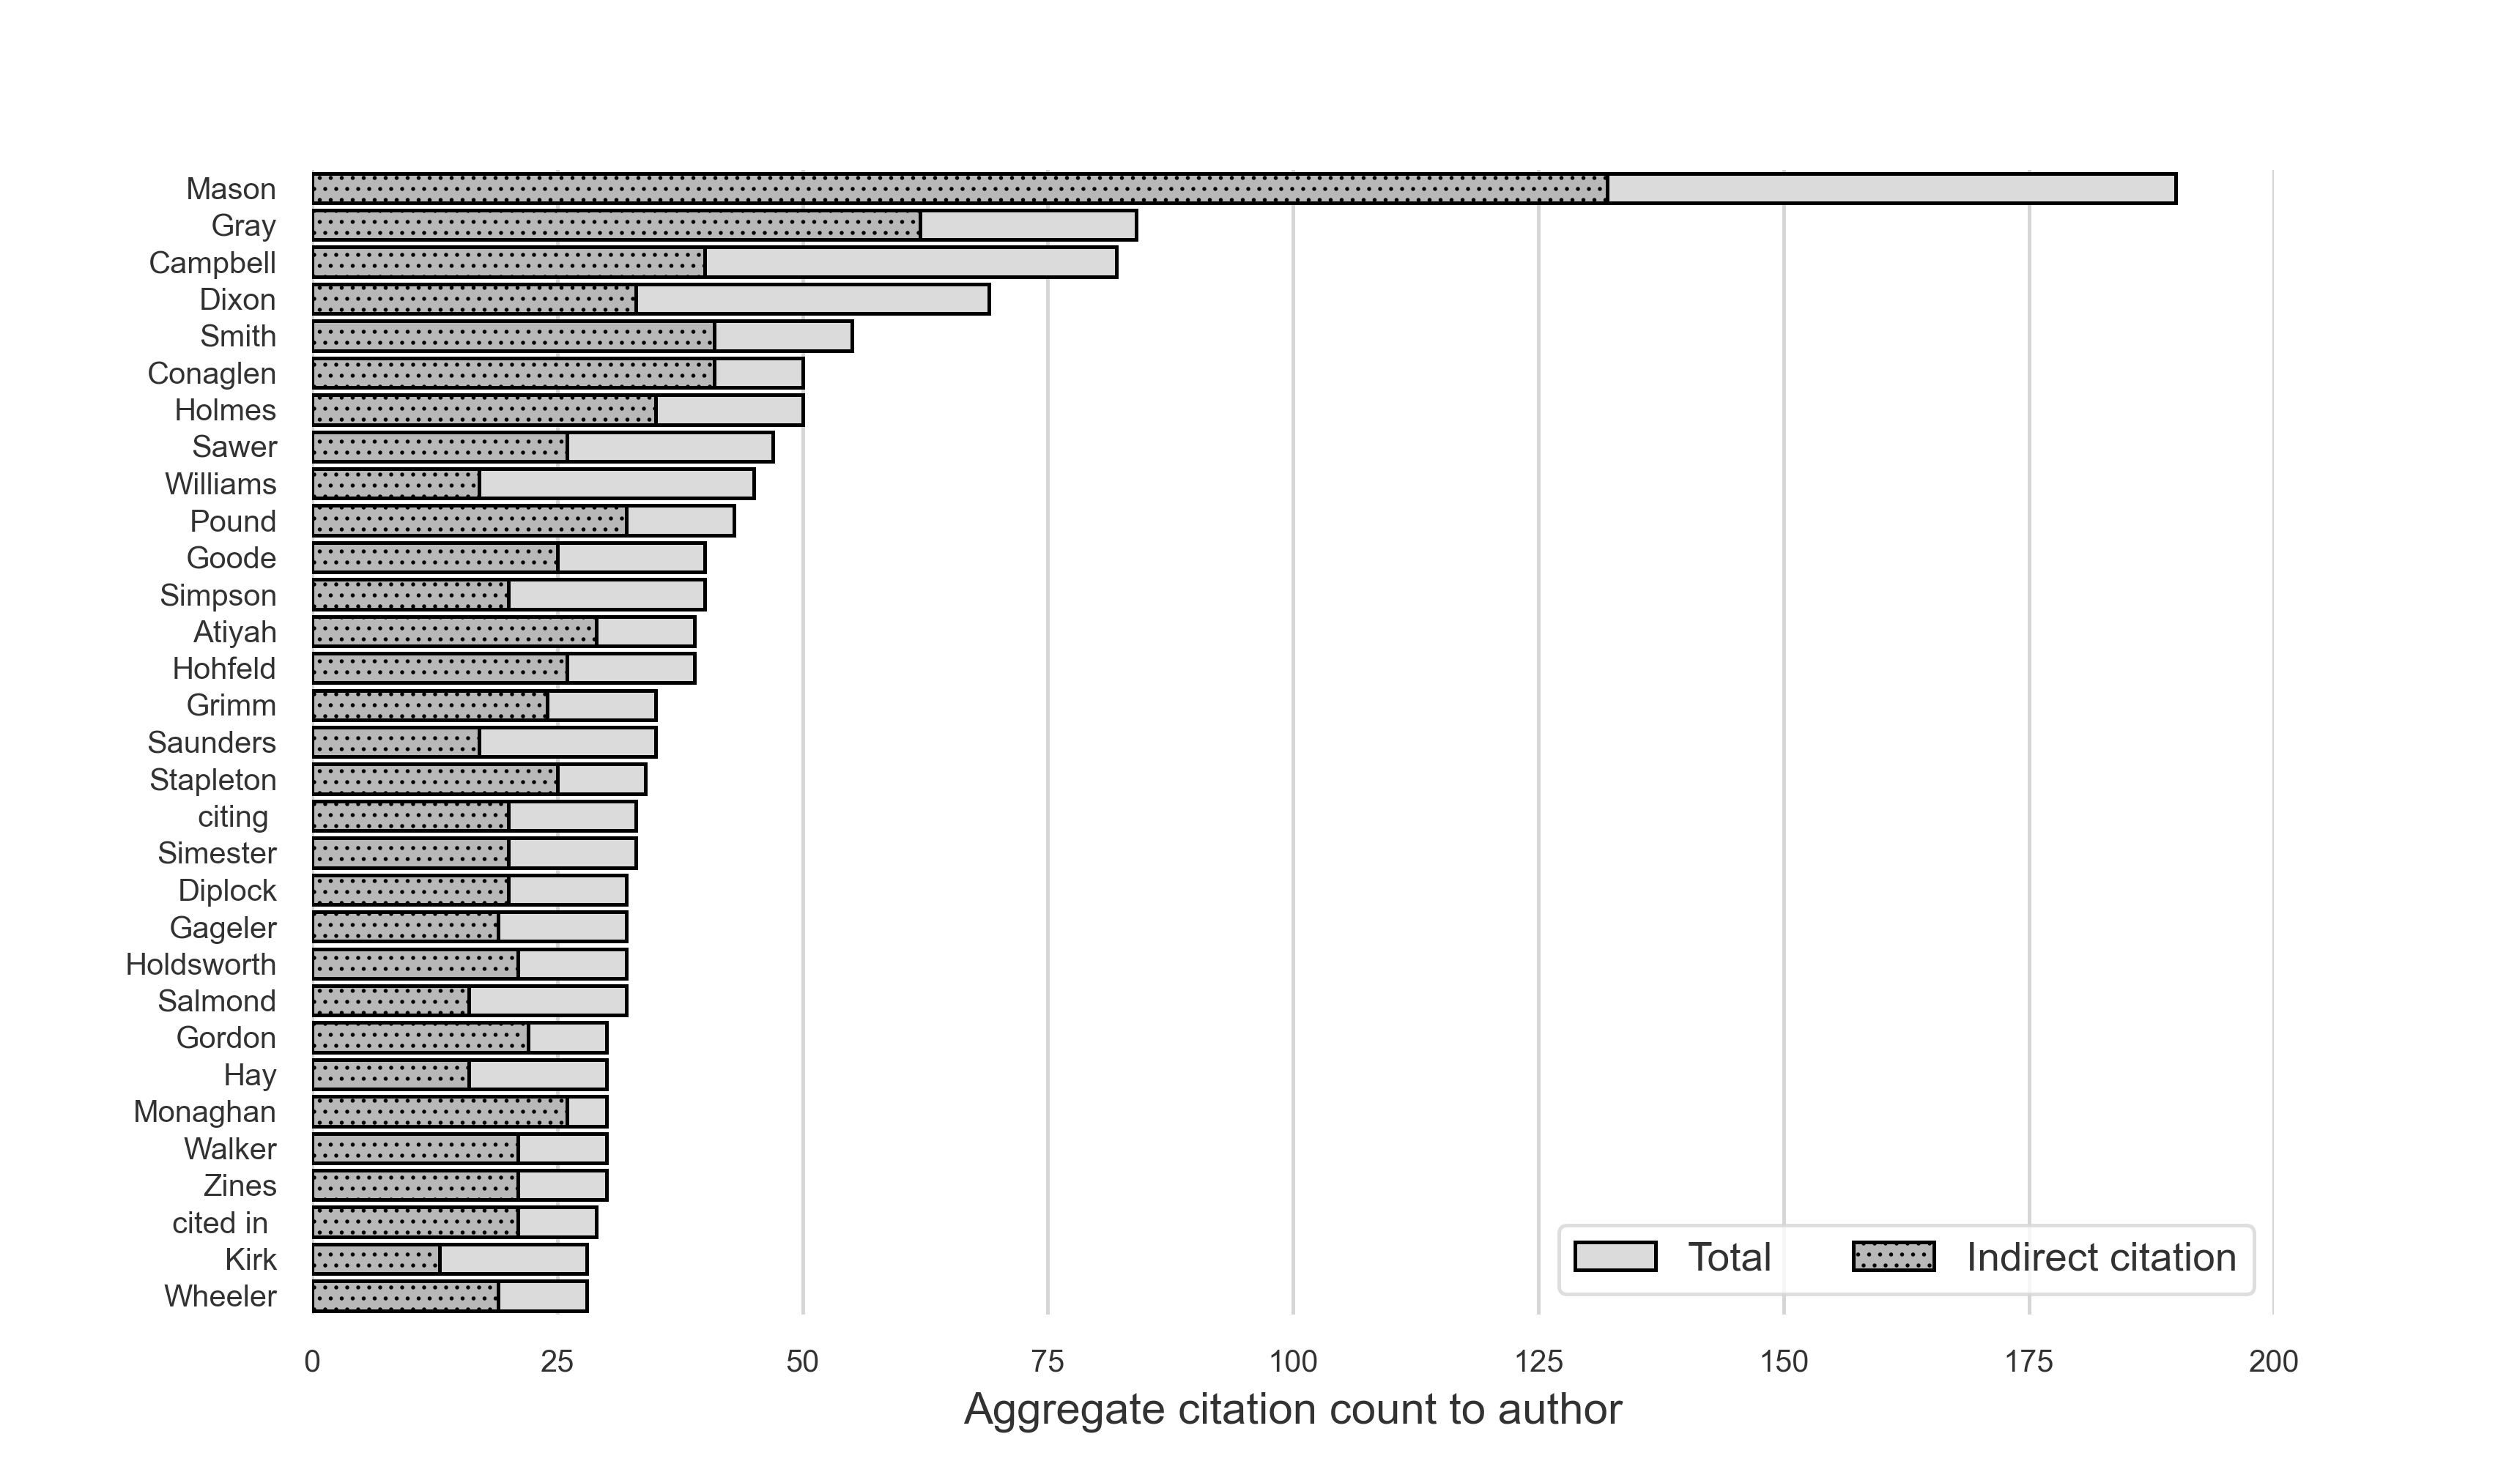
\includegraphics[]{Figs/authors.png}
%   \caption{fig.}
%   \label{fig:authors}
% \end{figure}

\let\xn\xnote
\renewcommand\thesubsubsection{RQ\arabic{subsubsection}}

\section{Evaluation}

\subsection{Research Questions}

\subsubsection{Are modern courts more open to citing secondary sources?}

\subsubsection{What influences the incidence of a citation to a secondary source?}

\subsubsection{Which academics influence the development of substantive law?}

\subsection{Limitations}

% Polarity of cited passage -- Negative citations -- But see (sceptically) Stephen J Choi and Mitu G Gulati, 'Choosing the Next Supreme Court Justice: An Empirical Ranking of
% Judge Performance' (2004) 78 Southern California Law Review 23, 56-7.

% What about minority opinions. See also Dickenson's Arcade Pty Ltd v Tasmania [1974] HCA 9; 130 CLR 177 at 188. Constructing authority from fragmented authority. But also see Federation Insurance Ltd v Wasson [1987] HCA 34; 163 CLR 303 at [17]. Consideration of dissenting judgments.

% Manual vs auto generated data sets.

% Time period?

\let\xn\xnote
\section{Conclusion and Future Work}

% Technical:
% Text classification to determine the polarity of a passage.
% Topic clustering using LDA / transformer based models.
% More data

% Legal:
% Network effect of citations to academics. Bandwagon effects and positive feedback loops?

\newpage
%TC:ignore
\section{Bibliography}

\subsection{\textit{Articles/Books/Reports}}

\subsection{\textit{Cases}}

\subsection{\textit{Legislation}}

\subsection{\textit{Other}}

%TC:endignore

\end{document}